\documentclass[a4wide]{report}

\usepackage{amsmath}
\usepackage[a4paper, total={7in, 10.2in}]{geometry}
\usepackage{graphicx}
\usepackage[portuguese]{babel}
\usepackage[utf8]{inputenc}

\begin{document}

\noindent
{\bf Lincoln Martins de Oliveira (ES 90693) - Mini-relatório 03 (\today)}

\begin{quote}

\centering

\bf Mini relatório referente ao exercício 1 e 2 das aulas 11 e 12

\end{quote}
\vspace{0.5cm}
\begin{quote}

\bf  exercício 1 :

\end{quote}

Este exercício nos apresenta um cicuito elétrico e através das Leis de Kirchhoff 
nos deu um sistema de equações que pode ser escrito na forma matricial.

\begin{quote}

\bf 01) a-

\end{quote}

Expressãanalítica para a matriz $\bf R$.
 \begin{Large}
\begin{equation} %excrevendo em forma de matricial
\bf R=\left[\begin{array}{ccc}
r_{s} & r_{1} & r_{2} \\
-r_{x} & r_{1} + r_{2} + r_{a} & -r_{a} \\
-r_{3} & -r_{a} & r_{2} + r_{3} + r_{a}
\end{array}\right]\quad
\label{matrizR}
\end{equation}
\end{Large}

\begin{quote}

\bf 01) b- 

\end{quote}

Considerando o método de decomposição LU (vaja em~\cite{Metodos}) 
para matrizes $n_{vs} n$, onde a matriz $\bf R$ é reescrita como a multiplicação 
das matrizes L e U. Escrevemos as expressões analíticas para matrizes L e U, ou seja,
explicitando como os seus elementos em função das resistências.
\begin{large}
\begin{equation} %excrevendo em forma de matricial
\centering
\bf U=\left[\begin{array}{ccc}
r_{s} & r_{1} & r_{2} \\
0 & r_{1} + r_{2} + r_{a}+(\frac{r_{3}}{r_{s}})r_{1} & -r_{a} \\
0 & 0 & u_{3 3}
\end{array}\right]\quad
\label{matrizU}
\end{equation}
\end{large}

Onde o elemento $u_{3 3}$ vale : 

\begin{large}
\begin{equation}
\centering
u_{3 3} = r_{2} + r_{3} + r_{a} + \frac{r_{3}}{r_{s}}r_{2} - \frac{r_{a}^{2}}{u_{22}}(\frac{r_{3}r_{1}r_{a}}{r_{s}})
\end{equation}
\end{large}


\begin{Large}
\begin{equation} %excrevendo em forma de matricial
\centering
\bf L=\left[\begin{array}{ccc}
1 & 0 & 0 \\
\frac{-r_{x}}{r_{a}} & 1 & 0 \\
\frac{-r_{3}}{r_{s}} & \frac{-r_{3}r{1}}{r_{s}u_{22}} -\frac{-r_{a}}{u_{22}} & 1
\end{array}\right]\quad
\label{matrizU}
\end{equation}
\end{Large}

\begin{quote}

\bf 01) c- 

\end{quote}

Aqui foi feito um programa para encontrar as correntes elétricas bastando apenas usuario entre 
com os valores das resistências e das voltagens ao final o programa exibirá a matriz das resistências 
e os valores das correntes $i_1$,$i_2$ e $i_3$,tal programa pode ser encontrado na pasta ex01c.

Observe que as respectivas resistências que devem ser introduzidas no programa estão abaixo, 
e as voltagens a serem inseridas (vaja em~\cite{roteiro}):


\begin{equation} %excrevendo em forma de matricial
\bf R=\left[\begin{array}{ccc}
10 & 100 & 100 \\
-120 & 1220 & -1000 \\
-150 & -1000 & 1250
\end{array}\right]\quad
\label{matrizR}
\end{equation}




\begin{quote}

\bf 01) d- 

\end{quote}

A corrente $i_a$ no amperímetro pode ser encontrada utilizando a consideração de Kirchhoff referente aos nós em um circuito.
Logo a corrente $i_a$ tem o valor de:

\begin{equation}
\centering
i_{2} = i_{3} + i_{a} \Rightarrow i_{a} = i_{2} - i_{3} \Rightarrow i_{a} = -6.865E-005
\label{correnteIa}
\end{equation}

A ponte estar balanceada significa que não passa qualquer corrente pelo anperímetro, como vimos que ha a passagem de corrente logo ela não está balanceada.

\begin{quote}

\bf  exercício 2 :

\end{quote}

Neste exercício nos foi proposto interpolar um conjunto de $n+1$ dados experimentais da forma $(x_{k},y{k})$
utilizando um polinômio p(x) de grau n impondo que $p(x_{k}) = y_{k}$ $\forall$ $k$ para podermos escrever um sistema
de aquações como proposto (vaja em~\cite{roteiro}).

\begin{quote}

\bf 02) a- 

\end{quote}

Utilizando o método de decomposição LU fiz um programa para encontrar os coeficiêntes $a_k$ da função polinomial p(x) que interpola
os dados experimentais do arquivo planck.dat. Tal programa pode ser encontrado na pasta 02a, nela tembém pode-se encontrar as matrizes 
L, U, X e os coeficiêntes angulares $a_k$ salvos em arquivos .dat.

\begin{quote}

\bf 02) b- 

\end{quote}

Aqui foi feito um gráfico com os dados experimentais e também com a curva da função polinomial p(x) encontrada no
item (a) dentro do intervalo x $\in $ [0.01, 1.0].

\begin{figure}[h]
\centering
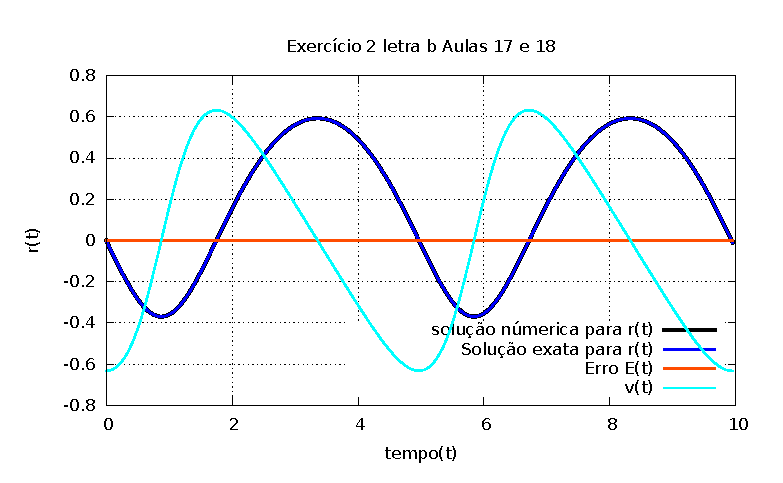
\includegraphics[width=0.5\textwidth]{ex02b}
\caption{Dados experimentais em azul e a curva descrita por p(x) no intervalo dado de x em vermelho.}
\label{ex02b1.1}
\end{figure}

\begin{quote}

\bf 02) c- 

\end{quote}

Fizemos um gráfico para comparar o polinômio p(x) encontrado com a função exata para a distribuição de Planck
dada por P(x)(vaja em~\cite{roteiro}):

\begin{figure}[h]
\centering
\includegraphics[width=0.5\textwidth]{ex02c}
\caption{curva descrita por p(x) em vermelho e função para a distribuição de Planck P(x) em preto.}
\label{ex02b1.2}
\end{figure}

\begin{quote}

\bf 02) d- 

\end{quote}

Expressões analíticas para as derivadas p'(x) e P'(x):

\begin{equation}
\centering
p'(x) = na_{n}x^{n-1} + (n - 1)a_{n-1}x^{n-2} ...  + 2a_{2}x^{1} + a_{1}x^{0}      
\label{plinha(x)1.1}
\end{equation}
\begin{equation}
\centering
P'(x)= - \frac{5x(e^{\frac{1}{x}} - 1) - e^{\frac{1}{x}} }{x^{7}(e^{\frac{1}{x}}-1)^{2}}
\label{Plinha(x)1.2}
\end{equation}

\begin{figure}[h]
\centering
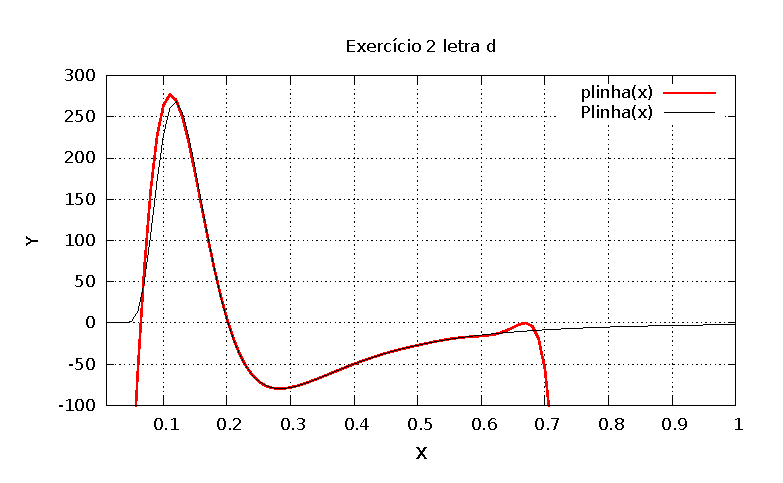
\includegraphics[width=0.5\textwidth]{ex02d}
\caption{curva descrita pela derivada de p(x) em vermelho (p'(x)) e a derivada da função para a distribuição de Planck P(x) em preto (P'(x)).}
\label{ex02d1.1}
\end{figure}

\begin{thebibliography}{99}

\bibitem{Metodos} C. Scherer. Metodos Computacionais da Física (2nd ed.,2010)

\bibitem{roteiro} AULAS 11 E 12: FIS-271 - Física Computacional I

\end{thebibliography}
\end{document}